\section{Motivations}
A volumetric display is a type of graphical display device that visually represents objects and scenes natively in 3D. These displays differ from more traditional virtual reality devices in that they are not immersive; rather, they coexist with their surroundings. They can be viewed from any angle without the need for special visual apparatus and can be observed by multiple people simultaneously \cite{1492264}. There is no real consensus on what exactly constitutes a volumetric display, let alone the best way to build one. As we cover in the Background \ref{sect:3d}, there are currently many approaches being explored by both academic and industrial research groups to develop these displays.

 
\begin{invisBox}
	\pictureBox[label={fig:medical-use}]{PerspectaRAD being used to view a CT image of a patient's head \cite{radiation-therapy}}{
	  \adjustbox{height=5.25cm, keepaspectratio}{
		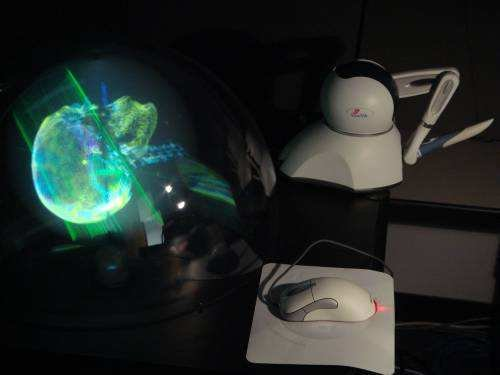
\includegraphics{./introduction/figures/medical-imaging.jpg}
	  }
	}
	\hfill
	\pictureBox[label={fig:graph-use}]{Graph Visualization on the Voxon Photonics VX1 \cite{noauthor_Voxon_community_nodate}}{
	\adjustbox{height=5.25cm, keepaspectratio}{
	  \includegraphics{./introduction/figures/graph.png}
	  }
	}
\end{invisBox}

Due to their capacity to display objects and scenes to multiple viewers simultaneously, volumetric displays have been applied to a variety of professional and academic fields, including but not limited to medical imaging \cite{Gong2009-vc} (see Fig~\ref{fig:medical-use}), scientific visualization (see Fig.~\ref{fig:graph-use}), computer-aided design \cite{stickland_development_2003}, and military visualization \cite{10.1117/12.785009} \cite{1492264} \cite{noauthor_bae_nodate}. \\

As volumetric displays become more advanced and accessible, they have the potential to revolutionize the way we interact with digital content, providing benefits over alternative mediums like Virtual Reality (VR) (see Background \ref{sect:3d}). However, the high cost and complexity of these devices have limited their adoption and hindered research into their usability in the past. \\

It is currently difficult to conduct human-computer interaction (HCI) research in the field of volumetric displays because these devices are not widely available and are prohibitively expensive, costing upwards of \$11,700 USD \cite{noauthor_products_nodate}. There have been attempts to create devices that simulate volumetric displays to address this issue (see Background \ref{sect:3d}), but these solutions are often complex and expensive to replicate.

\section{Contributions}

Our project makes two novel contributions to the field of volumetric displays. Firstly, we built a system for simulating volumetric displays for use in HCI research. Secondly, we utilized our device to conduct a user study that successfully demonstrated the research viability of our system.

\begin{invisBox}
	\pictureBox[label={fig:volsim}]{Our simulator rendering Imperial College London in 3D}{
	  \adjustbox{height=8.0cm, keepaspectratio}{
		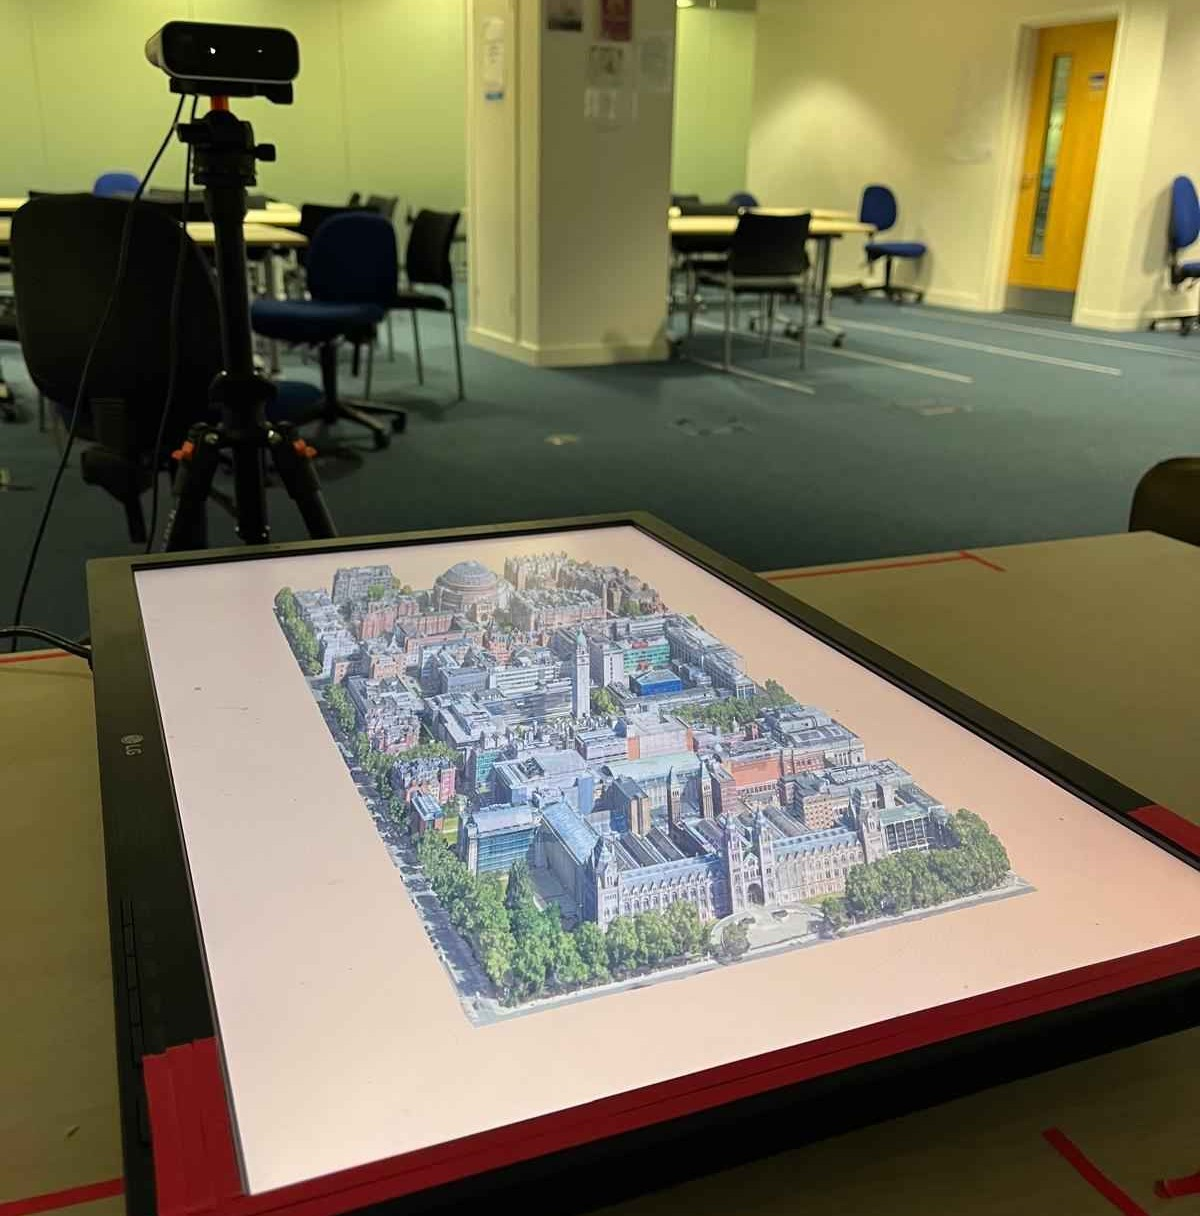
\includegraphics{./introduction/figures/volsim.jpg}
	  }
	}
	\hfill
	\pictureBox[label={fig:pov}]{POV perspective completing a task our user study}{
	\adjustbox{height=8.0cm, keepaspectratio}{
	  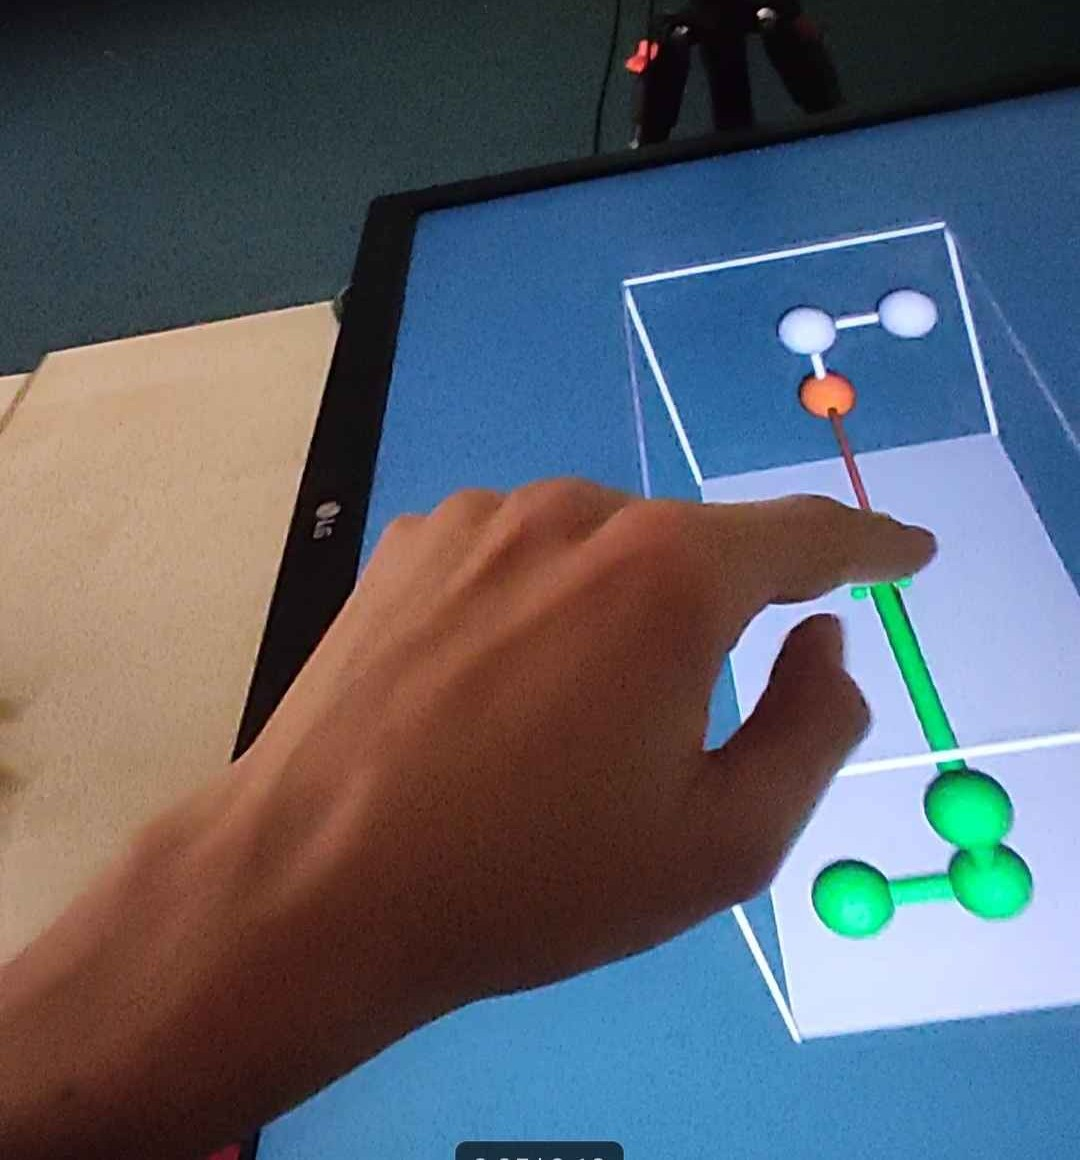
\includegraphics{./introduction/figures/pov-user-study.jpg}
	  }
	}
\end{invisBox}

\subsubsection{Volumetric Display Simulator}
We created our Volumetric Display Simulator (see Implementation \ref{sect:overview}) with the intention of forming a strong foundation for conducting future user studies involving volumetric displays. \\

Our simulator (as seen in Fig~\ref{fig:volsim}) uses head tracking to render the correct perspective for the viewer using the device. This allows the user to change the view while maintaining the illusion of a 3D scene in front of them. We also implemented native hand tracking integration, allowing the user to interact with the scene using their hands, which to our knowledge makes our device the first to support such a feature. \\

We designed our system in a such a way that it is: 

\begin{enumerate}
    \item \textbf{Cost-Effective:} The system was designed to operate on a standard desktop computer with regular monitors using common hardware. It utilizes Microsoft's widely used Azure Kinect Camera for its head and hand tracking. We believe our system's affordability and accessibility will encourage more researchers to explore volumetric display technology.

    \item \textbf{Reproducible:} The system was developed using Nix (see Background \ref{sect:nix}), a package manager that facilitates the easy reproduction and compilation of software environments. This means the system can be run on any computer with Nix installed using a single command (see Implementation \ref{sect:buildsystem}). This not only simplifies execution but also enhances the ease of sharing and reproducing results.

    \item \textbf{Simple and Lightweight:} The system was intentionally designed to be as simple as possible by leveraging well-established libraries (see Implementation \ref{sect:renderer} and Implementation \ref{sect:tracker}). The simulator comprises only approximately 2,000 lines of C++ code, making it straightforward to understand and modify. We hope that this simplicity will encourage other researchers to build upon our work and develop new features.
\end{enumerate}

\subsubsection{User Study}

We conducted a full user study to validate the effectiveness of our simulator. Our aim was to demonstrate that our system could be used to conduct meaningful research into the usability of volumetric displays. \\

We chose to investigate the performance of participants in a task that required them to trace a path with their hands under different conditions (see Implementation \ref{sect:userstudy}). An example of the task can be seen in Fig.~\ref{fig:pov}. We focused on two factors: the perspective of the display (2D vs. 3D) and the method of interaction (direct hand interaction vs teleoperation), resulting in a total of four conditions. \\

The findings indicated that using head tracking for a 3D perspective significantly improved task completion speed and accuracy compared to a 2D display. Additionally, direct hand interaction with the volumetric display yielded superior results compared to teleoperation, particularly when paired with a 3D view. \\

We observed a strong user preference for the 3D perspective while using direct hand interaction, suggesting that users value natural and intuitive interaction modes. The findings reaffirm the advantage of motion parallax in 3D tasks, showing that the benefits of 3D tracking are diminished with positional offsets. \\

The study identifies several areas for further investigation, including the effects of varying offset distances and the potential impact of offsetting the interaction zone rather than the display itself. These recommendations can guide future research efforts to refine and improve the usability of volumetric displays. (For more information see Evaluation \ref{sect:eval-userstudy}).

